%%%%%%%%%%%%%%%%%%%%%%%%%%%%%%%%%%%%%%%%%%%%%%%%%%%%%%%%%%%%%%%%%%%%%%%%%
%                           Marco Conceptual                               %
%%%%%%%%%%%%%%%%%%%%%%%%%%%%%%%%%%%%%%%%%%%%%%%%%%%%%%%%%%%%%%%%%%%%%%%%%

\chapter{Marco conceptual}\label{chapter2}
El presente Trabajo Terminal tiene como objetivo el desarrollo de un prototipo de aplicación para el sistema operativo Android que permita la clasificación de las gasolineras de la Ciudad de México a partir de la implementación de un algoritmo computacional, el cuál, utilizará las mediciones de diferentes sensores de flujo los cuáles enviarán sus datos a través de un módulo Bluetooth.
\paragraph{}
Dado que este trabajo terminal emplea conceptos de diversas áreas de la Ingeniería en Sistemas Computacionales, resulta fundamental dar una serie de definiciones previas que permitan un mejor entendimiento del documento.

\section{Gasolineras y su funcionamiento}
Primeramente, es necesario conocer los conceptos relacionados con una gasolinera, así como el estado actual de estos establecimientos en nuestro país.
\paragraph{}
Comenzaremos con la definición de gasolinera o estación de servicio. En el español general, la voz más usual para referirse al ‘depósito de gasolina para la venta al público’ o al ‘establecimiento donde se vende gasolina’ es gasolinera \citep{MarcoTeorico1}. 

Una vez que se ha identificado el concepto de gasolinera podemos empezar a citar datos estadísticos que concuerden con estos establecimientos, a continuación, se citan algunas cifras importantes que nos dan un panorama del número de gasolineras en el país y su relación con respecto al número de automóviles en circulación. En el año 2017 se registraron más de 12,000 gasolineras en todo México, estos establecimientos dan servicio a aproximadamente 43 millones de vehículos en circulación, es decir,  que cada gasolinera debe abastecer a cerca de 3,652 vehículos.  Traducido de otra forma, hay en promedio una gasolinera por cada 10 mil 514 habitantes, de acuerdo a la Comisión Reguladora de Energía (CRE)\citep{MarcoTeorico2}.
\paragraph{}
Siendo un poco más específicos, en la Ciudad de México hay 4.6 millones de autos y menos de 500 estaciones de servicio, así, cada gasolinera debe atender en promedio a 11 mil 400 vehículos. Una de las principales razones por las cuáles el número de gasolineras resulta relativamente bajo tiene que ver con las normas que rigen la construcción y mantenimiento de las Estaciones de Servicio en México \citep{MarcoTeorico2}, pues los requerimientos necesarios para la creación de una nueva gasolinera son numerosos. Es así, que resulta importante estudiar los normas para la construcción y operación de las gasolineras en México.

\paragraph{NOM-005-ASEA-2016}
En México, la norma que rige el diseño, construcción, operación y mantenimiento de Estaciones de Servicio para almacenamiento y expendio de diésel y gasolinas en la NORMA Oficial Mexicana NOM-005-ASEA-2016, la cual, es emitida por la Agencia Nacional de Seguridad Industrial y de Protección al Medio Ambiente del Sector Hidrocarburos. Dicha norma tiene como objetivo establecer las especificaciones, parámetros y requisitos técnicos de Seguridad Industrial, Seguridad Operativa, y Protección Ambiental que se deben cumplir en el diseño, construcción, operación y mantenimiento de Estaciones de Servicio para almacenamiento y expendio de diésel y gasolinas.

Tomando como referencia la NOM-005 daremos una introducción a los elementos que se usan dentro de una gasolinera para el proceso de suministro y recarga de combustible.
El proceso de suministro de gasolina comienza cuando un vehículo accede a una estación de servicio y realiza una maniobra de frenado junto a un módulo de despacho. Según la NOM-005 un módulo de despacho es un elemento junto al cual el vehículo o embarcación se abastecen de combustible a través de un dispensario. El dispensario o expendedor de gasolina es el sistema automático usado para la medición y despacho de gasolina y otros combustibles líquidos \citep{NORMA-005}.
Posteriormente, personal competente realiza transmisión de combustible del expendedor de gasolina al tanque del automóvil para que finalmente, el usuario realice el pago correspondiente por la cantidad de combustible que fue ingresado al vehículo.

\paragraph{El dispensador de combustible}
Ahora que se ha definido el proceso de suministro de gasolina, es necesario definir algunos de los elementos que intervienen en él, se hará énfasis en aquellos conceptos relacionados con la medición de combustible, ya que esta variable influye de manera directa en el presente trabajo.

Históricamente, el primer dispensador de combustible fue creado por Sylvanus Bowser el 5 de septiembre de 1885 en Indiana Estados Unidos \citep{MarcoTeorico4}. Dicho dispensador no era usado para para automóviles debido a la poca comercialización que existía, en su lugar era utilizado para recargar lámparas de keroseno y estufas. El primer dispensador de combustible fue patentado por el noruego John J. Tokheim en 1901. El gigante de la industria minorista de combustibles Tokheim-OPW, recibió su nombre es honor a este científico. \citep{MarcoTeorico4}

El elemento principal para el suministro de gasolina es el dispensador de combustible, el cuál, se compone de dos partes principales: la unidad de control electrónica, que contiene un sistema embebido para controlar la acción de la bomba y que se comunica con el sistema del mostrador, y en segundo lugar, una sección mecánica que contiene una bomba eléctrica y unas válvulas para bombear físicamente el combustible. 
\\Los dispensadores más modernos están equipados normalmente con un sistema de control de recuperación de vapores, para evitar que los vapores de la gasolina se escapen hacia el aire de la gasolinera.

A lo largo de la historia, los dispensadores de combustible han tenido una gama muy amplia de diseños para resolver los problemas mecánicos del bombeo, la medición confiable, la seguridad y la estética.\\\\

En la Figura \ref{fig:diagrama_dispensador} se observa un diagrama general de un dispensador de combustible.
\begin{figure}[H]
	\centering
	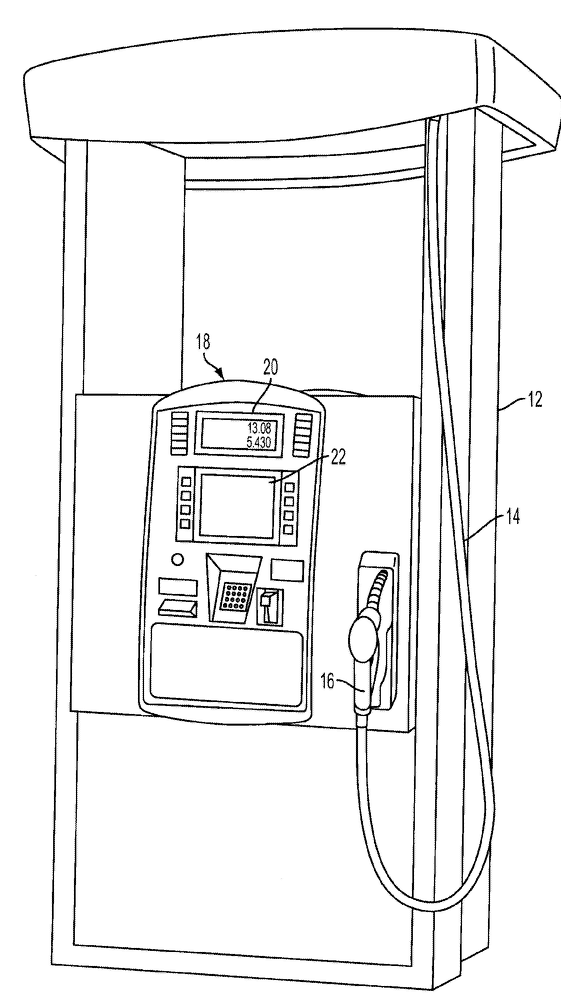
\includegraphics[scale=.25]{Capitulo2/images/diagrama_dispensador}
	\caption{Patente de dispensador de combustible}
	\label{fig:diagrama_dispensador}
\end{figure}

\paragraph{Mediciones de un dispensador de gasolina}
Una de las funciones más importantes de una del dispensador de combustible en una estación de servicio, es la medición precisa y consistente del flujo y volumen despachado. Esta medición es realizada comúnmente por un medidor volumétrico de operación mecánica, conectado a un panel electrónico que contabiliza el volumen y realiza la conversión hacia la moneda local para finalmente cobrar al consumidor \citep{MarcoTeorico3}.

\paragraph{Medidor de compresión de pistones}La medición de flujo casi siempre se realiza mediante un medidor de 4 pistones conectado a un codificador electrónico. Las bombas de combustible convierten el movimiento del medidor en impulsos eléctricos utilizando un codificador rotatorio \citep{MarcoTeorico5}.

\begin{figure}[H]
	\centering
	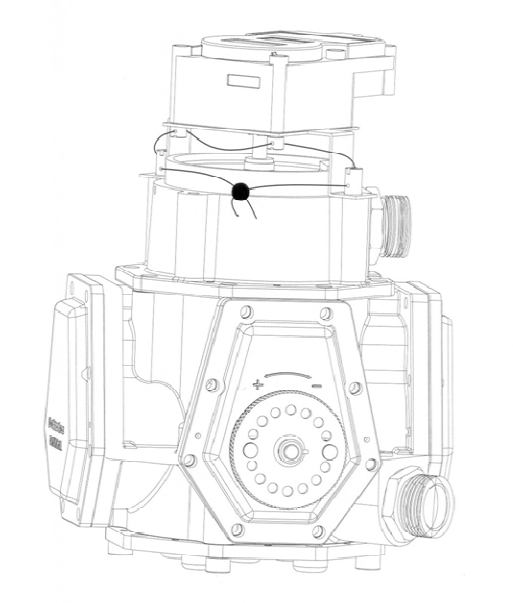
\includegraphics[scale=.4]{Capitulo2/images/medidor_gasolina}
	\caption{Medidor de 4 pistones de la empresa Petrotec}
	\label{fig:medidor_gasolina}
\end{figure}

\paragraph{Codificador rotatorio}
Un codificador rotatorio es un dispositivo electromecánico que convierte la posición angular de un eje, directamente a un código digital, estos dispositivos son considerados como transductores \citep{MarcoTeorico6}.

\begin{figure}[H]
	\centering
	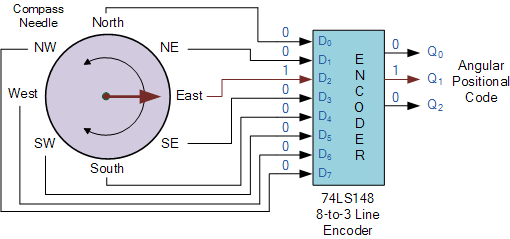
\includegraphics[scale=.8]{Capitulo2/images/electronic_encoder}
	\caption{Diagrama interno de un codificador rotatorio}
	\label{fig:electronic_encoder}
\end{figure}

\paragraph{Sistema embebido del dispensador}
Una vez que el codificador rotatorio ha empezado a registrar un movimiento angular los impulsos que éste emite son enviados al sistema embebido del dispensador de combustible, dicho sistema se encarga de realizar el cómputo de las señales recibidas, el estudió de esta unidad computacional resulta extenso ya que es el encargado de realizar toda la parte electrónica del dispensador de gasolina, por lo que a continuación se muestra una imágen de una placa que la empresa Gasboy utiliza para los dispensadores de gasolina que comercializan.

\begin{figure}[H]
	\centering
	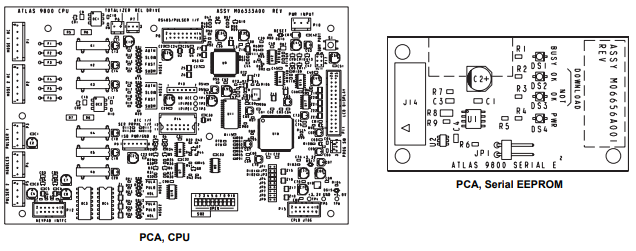
\includegraphics[scale=.8]{Capitulo2/images/pca_gasboy}
	\caption{Printed Circuit Assembly de la empresa Gasboy para dispensadores de gasolina}
	\label{fig:pca_gasboy}
\end{figure}

\paragraph{Pistola de combustible}
Las pistolas están conectadas a la bomba a través de mangueras flexibles, lo que permite colocarlas en la entrada de llenado del vehículo. Las mangueras son robustas para resistir el desgaste intenso, incluida la exposición a la intemperie y el arrastre, y a menudo se unen utilizando resortes pesados o arreglos de bobina para proporcionar resistencia adicional.

\begin{figure}[H]
	\centering
	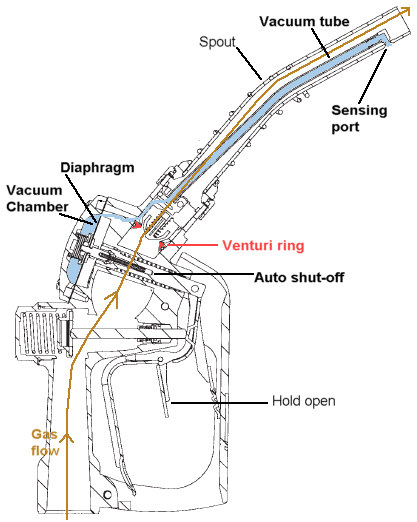
\includegraphics[scale=.6]{Capitulo2/images/nozzle}
	\caption{Pistola de combustible y sus componentes}
	\label{fig:nozzle}
\end{figure}

A continuación se enlistan los pasos que describen el funcionamiento de una pistola de combustible, además se muestra una tabla con las características técnicas de una pistola de la marca estadounidense Husky.

\begin{itemize}
	\item El dispensador es activado presionando el pivote con la marca Hold open.
	\item La pistola de combustible se encuentra presurizada y la gasolina empieza a fluir a través del cuerpo de la pistola.
	\item La gasolina entra en contacto con el anillo Venturi y provoca que la válvula contra derrames sea activada.
	\item Mientras la gasolina fluye a través del cuerpo de la pistola el tubo de vacío (Vacuum tube en la figura) aspira aire debido a un efecto de baja presión.
	\item Cuando el nivel de gasolina cubre el área de la figura marcada como Sensing port este no puede seguir ingresando aire lo que provoca que el diafragma sea activado cerrando el paso de gasolina.
\end{itemize}

\paragraph{Funcionamiento de una pistola de combustible}
Los pasos listados anteriormente fueron obtenidos de un vídeo hecho por el presidente de la Compañia Husky, Grenville Sutcliffe, dicho recurso puede ser consultado en el link de la cita correspondiente \citep{MarcoTeorico8}.
\paragraph{}
Especificación de una pistola de combustible de la Marca Husky
\begin{longtable}{|M{7cm}|M{7.5cm}|}
	\hline
	\textbf{Característica} & \textbf{Valor}
	\\\hline
	Tipo & Husky X-Mate
	\\\hline
	Material & Cuerpo de alumino, Recubrimiento de teflón, Sellos de Viton,
	Vástago de acero inoxidable
	\\\hline
	Rango de flujo & 8~60 litros/min
	\\\hline
	Diametro del canal & 20.6mm (13/16th")
	\\\hline
	Presión(min) & 2.4 PSI (160mBar)
	\\\hline
	Presión(max) & 50 PSI (3.35Bar)
	\\\hline
	Rango de temperatura & -6 C to +55 C
	\\\hline
	Conexiones & 3/4 BSP(F)
	\\\hline
	\caption{Características de una pistola de combustible}
	\label{tabla_pistola_combustible} 
\end{longtable}

\paragraph{Consideraciones para la medición}
En los EE. UU., la cantidad de flujo está limitada a 10 galones por minuto (37.9 litros) para automóviles y 40 galones por minuto para camiones. Este caudal se basa en el diámetro del tubo de llenado de combustible del vehículo, que limita el flujo a estas cantidades. Aunque la medidas de velocidad de flujo anteriores fueron determinadas por el National Institute of Standards and Technology de los Estados Unidos, éstas serán utilizadas en el presente trabajo, ya que los modelos de los automóviles que fueron usados para las pruebas tienen una presencia mayoritaria en nuestros país \citep{MarcoTeorico7}.
\paragraph{}
Derivado de lo anterior se deberá buscar un sensor que soporte las mismas especificaciones de presión, cantidad de flujo y pulsos de salida que los componentes que conforman a dispensador de gasolina, esto con la finalidad de obtener mediciones lo más cercanas posibles a la realidad al momento de implementar nuestro proyecto.
\section{Sensores}
En la sección anterior observamos que para hacer la mediciones de los litros de gasolina que son ingresados a un automóvil se hace uso de diferentes sensores. De igual forma, en el objetivo del presente trabajo se plantea el uso de un sensor de flujo para las mediciones en el proceso de suministro de gasolina, es por eso, que a continuación se define el concepto de sensor.
\\
Los sensores, son los elementos que se encuentran en contacto con una planta, y tienen una salida que depende de alguna manera de la variable que está siendo medida o monitoreada \citep{MarcoTeorico10}. Si existe más de un elemento de sensado o monitoreo dentro del sistema, él elemento que se encuentre en contacto directo con la planta generadora de las variables recibe el nombre de “elemento principal de medición”, lo otros son elementos secundarios de medición.
\\
Un sensor es todo aquello que tiene una propiedad sensible a una magnitud del medio, y al variar esta magnitud también varia con cierta intensidad la propiedad, es decir, manifiesta la presencia de dicha magnitud, y también su medida.

\subsection{Sensor de flujo}
La medición de la tasa de flujo de un material a través de tuberías es extremadamente importante en
una amplia gama de industrias, incluyendo la industria química, del petróleo, del acero, de alimentos servicios públicos, entre otros. \citep{MarcoTeorico10}
Hay un gran número de medidores de flujo en el mercado. 
\\
El sensor de flujo es un dispositivo que, instalado en línea con una tubería, permite determinar cuándo está circulando un líquido o un gas. Estos son del tipo apagado/encendido ya que  determinan cuándo está o no circulando un fluido, pero no miden el caudal. Para medir el caudal se requiere un caudalímetro.

\begin{figure}[H]
	\centering
	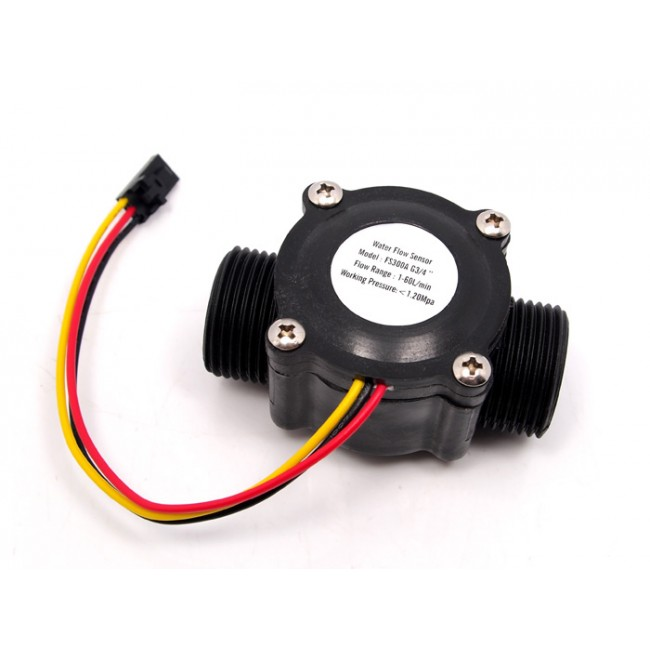
\includegraphics[scale=.4]{Capitulo2/images/flowmeter}
	\caption{Sensor de flujo de Efecto Hall}
	\label{fig:flowmeter}
\end{figure}

\paragraph{Caudalímetro}
Un caudalímetro es un instrumento de medida para la medición de caudal o gasto volumétrico de un fluido. También suelen llamarse medidores de caudal, medidores de flujo o flujómetros \citep{MarcoTeorico10}.

A continuación, se muestra una lista con los tipos de caudalímetros más comunes en el mercado:
\begin{itemize}
	\item Caudalímetro de diferencial de presión. Estos son los caudalímetros industriales más comunes para líquidos y gases limpios. \citep{MarcoTeorico10}
	\item Caudalímetro Mecánico. Consisten en un molino cuyas aspas están transversales a la circulación de fluido. El flujo hace girar el molino cuyo eje mueve un contador que acumula lecturas.
	\item Caudalímetro Vortex
	\item Caudalímetro Mecánico
\end{itemize} 
\section{Comunicación inalámbrica}
\subsection{Protocolo Bluetooth}
Bluetooth es una tecnología de conectividad inalámbrica de baja potencia que se utiliza para
transmitir audio, transferir datos y transmitir información entre dispositivos. Hay dos sabores
de la tecnología Bluetooth, velocidad básica / velocidad de datos mejorada (BR / EDR) y baja
energía (LE) \citep{Bluetooth}.
\subsection{WiFi}
WiFi es la abreviatura o el nombre comercial de Wireless Fidelity y, como su nombre lo indica,
es un sistema de conexión de ordenadores completamente inalámbrico, que permite a sus usuarios
compartir y transferir información utilizando ondas de radio, es decir, sin utilizar cableado alguno.
De esta manera, podemos mantener comunicaciones entre ordenadores, portátiles, móviles y otros
dispositivos que cuenten con tecnología de recepción inalámbrica, facilitando enormemente las
comunicaciones, incluso en lugares abiertos lejos de nuestras casas y ocinas. Las redes WiFi por
lo general son de libre acceso, a menos que estén protegidas mediante contraseñas, lo cual, indicará
que son unas redes privadas utilizadas para conexiones con redes locales (LAN)\citep{WiFi}.
%\subsection{Módulo Bluetooth}
%\subsection{Protocolo HTTP}
%\section{Aplicación Móvil}
%\subsection{Sistema Operativo Android}
\section{Arquitectura de microservicios}
A continuación, se presentan los conceptos más importantes de la arquitectura de software que será utilizada para el presente proyecto, la cuál, recibe el nombre de Arquitectura de Microservicios.
\paragraph{Patrón de arquitectura}
Los patrones arquitectónicos, o patrones de arquitectura, también llamados arquetipos ofrecen soluciones a problemas de arquitectura de software en ingeniería, además, ayudan a definir las características básicas y de comportamiento de una aplicación. Por ejemplo, algunos patrones de arquitectura naturalmente se prestan hacia aplicaciones altamente escalables, mientras que otros patrones de arquitectura se prestan naturalmente hacia aplicaciones que sean altamente ágiles \citep{MarcoTeorico9}.
\\
Actualmente, existen diversos patrones de arquitectura de software, enseguida, se listan algunos de los más populares:
\begin{itemize}
	\item Arquitectura N-capas
	\item Arquitectura Orientada a Eventos
	\item Arquitectura Micro-kernel
	\item Arquitectura de Microservicios
\end{itemize}

\paragraph{}
En la actualidad, la Arquitectura de Microservicios está ganando terreno rápidamente en la industria como una alternativa viable a las arquitecturas monolíticas y orientadas a servicios \citep{MarcoTeorico9}.

\paragraph{Component decoupling}
El primer concepto importante dentro de la arquitectura de microservicios es el de 'Separately deployment units'. Este concepto nos dice que dentro de una aplicación de software, se debe buscar es desacoplamiento de los componentes, de manera que cada unidad mínima de funcionalidad pueda ser puesta en producción de manera independiente, y sin que esta afecte a otras unidades.

\paragraph{Service component} Quizás el concepto más importante para entender con este patrón, es la noción de un componente de servicio. Estos componentes pueden variar en tamaño o granularidad (independencia con otros componentes), yendo desde un módulo sencillo hasta ocupar una gran parte de la aplicación. 
\\
Los componentes de servicio contienen uno o más módulos (por ejemplo, clases de Java) que representan una funcionalidad del sistema (por ejemplo, proporcionar el clima para un determinado
ciudad o pueblo). Diseñar el nivel correcto de granularidad de un componente de servicio es uno de los mayores retos dentro de una arquitectura de microservicios \citep{MarcoTeorico9}.

\paragraph{Distributed architecture}
Todos los componentes de esta arquitectura se encuentran totalmente desacoplados, además, son accedidos a través de un mecanismo de control de acceso remoto como REST, SOAP o RMI.

La naturaleza distribuida de este patrón de arquitectura es la forma en que logra su escalabilidad y características de despliegue superiores a las de otras arquitecturas \citep{MarcoTeorico9}.

\begin{figure}[H]
	\centering
	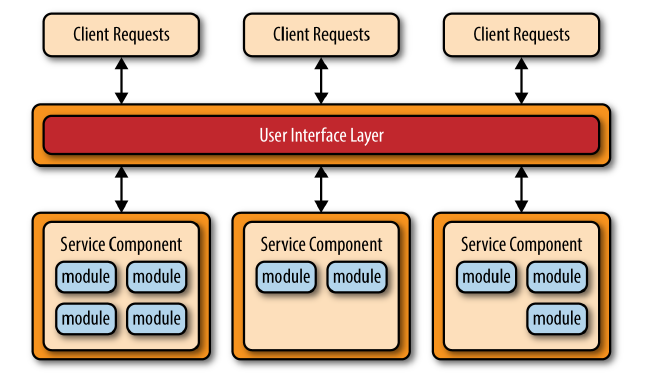
\includegraphics[scale=.6]{Capitulo2/images/microservicios}
	\caption{Arquitectura básica de microservicios}
	\label{fig:microservicios}
\end{figure}

\paragraph{Avoid dependencies and orchestration}
Uno de los principales retos de la arquitectura de microservicios es determinar el valor correcto de granularidad para los componentes de servicio. Si los componentes tienen un alto acoplamiento entre ellos, los beneficios de esta arquitectura no podrán ser aprovechados, por otro lado, si los componentes tiene una granularidad muy alta será necesario agregar un servicio de administración para dichos componentes llamado Orchestration. El problema de una granularidad alta, radica en que los diferentes servicios necesitarán una forma de comunicarse entre ellos, este fenómeno recibe el nombre de Interservice Communication, y provoca un alto acoplamiento entre componentes \citep{MarcoTeorico9}.
\\
Una forma de solventar el alto acoplamiento es mediante una base datos compartida entre los diferentes servicios de la aplicación.

\subsection{API REST}
Una API REST es una interfaz de comunicación basada en un conjunto de restricciones que permiten la comunicación maquina a maquina, el presente trabajo plantea el uso de un API REST por lo que es importante definirla y dar un contexto general de su uso.

\paragraph{Web service} Para poder definir un API REST es necesario dar un conjunto de conceptos previos. Un término que sale a relucir al hablar del tema es el de Servicio Web.
\\
Un servicio web es un término genérico para una función de software interoperable de máquina a máquina que se aloja en una dirección accesible de la red \citep{MarcoTeorico11}.
\\
Un servicio web, tiene una interfaz que oculta los detalles de su implementación, de esta forma, podrán usarse de forma independientemente de la plataforma de hardware o software en la que se haya implementado, e independientemente del lenguaje de programación en el que está escrito. Esta independencia fomenta que las aplicaciones basadas en servicios web tengan un bajo acoplamiento, sean orientadas a componentes, y permitan la comunicación entre diferentes tecnologías \citep{MarcoTeorico11}.

\begin{figure}[H]
	\centering
	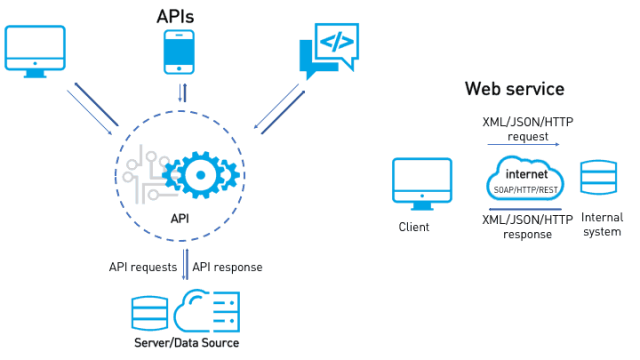
\includegraphics[scale=.6]{Capitulo2/images/web_service}
	\caption{Ejemplo de uso de los web services}
	\label{fig:web_service}
\end{figure}

En la actualidad, existen dos protocolos que son ampliamente usados para la implementación de servicios web:
\begin{itemize}
	\item SOAP (Simple Access Object Protocol)
	\item Protocolos JSON 
\end{itemize}

\paragraph{SOAP}
Un servicio web basado en SOAP posee una interfaz de comunicación descrita en un formato conocido como Web Service Definition Language (WSDL). A su vez, un servicio web SOAP es escrito usando una notación formal de XML, esta notación posee diversa información como Formatos de Mensaje, Protocolos de transporte y Ubicación. Existen herramientas que pueden ser usadas para procesar un WSDL y producir programas cliente capaces de comunicarse con el servicio utilizando el protocolo SOAP basado en XML. Aunque SOAP puede ser un protocolo de comunicación detallado, tiene la ventaja de la extensibilidad y esto hace que sea altamente usado en entornos empresariales \citep{MarcoTeorico11}.

\paragraph{JSON}
Un servicio web basado en el formato JSON utiliza el protocolo HTTP para establecer una comunicación, este protocolo es considerado menos formal que el uso del protocolo SOAP. Este tipo de servicios web es utilizado comúnmente para la comunicación con aplicaciones móviles gracias a la sencillez del protocolo \citep{MarcoTeorico11}.
 
\paragraph{Contraste}En contraste, un servicio web basado en SOAP agregar una capa de extensibilidad que es ideal para aplicaciones empresariales, pero pagando el precio de ser un protocolo bastante robusto y formal a la hora de escribir sus definiciones lo que implica un costo elevado de análisis y desarrollo, por otro lado, un servicio web basado en JSON permite un desarrollo ágil al utilizar un protocolo relativamente ligero como HTTP, sin embargo, su misma sencillez evita una formalidad al momento de adaptarlo al negocio, por lo que es recomendable utilizarse como puente de comunicación entre dispositivos.

Diferencias entre servicios web SOAP vs JSON \citep{MarcoTeorico11}:

\begin{itemize}
	\item El contenido de un mensaje SOAP esta en formato XML, mientras que un mensaje JSON contiene datos en formato JSON. JSON y XML son diferentes mecanismos de codificación para describir datos estructurados.
	\item JSON es un mecanismo de codificación bastante eficiente, por lo que los mensajes escritos tienden a ser mucho más pequeños que sus mensajes equivalentes en XML.
	\item JSON es un formato muy usado para aplicaciones móviles debido a su integración con Javascript, es por eso que es el mecanismo ideal para apps móviles.
	\item SOAP proporciona un mecanismo para agregar encabezados a un mensaje y una familia de especificaciones para la calidad del servicio (como la configuración de seguridad y las transacciones distribuidas). JSON no proporciona este mecanismo. En su lugar, se basa en los servicios del protocolo de red HTTP subyacente.
	\item Los servicios web basados en SOAP son descritos mediante un documento WSDL.
	\item Los servicios web SOAP tienen un formato de error explícito que implica el uso de mensajes de error SOAP. No hay equivalente para JSON.
	\item Los servicios web de JSON son compatibles tanto con una interfaz RESTful como con una interfaz Request-Response, SOAP solo es compatible con la interfaz de Request-Response. 
\end{itemize}

\paragraph{REST}
Una vez que hemos definido un servicio web y los tipos que existen actualmente, tenemos que crear un interfaz que nos permita implementar dichos servicios. Esta interfaz permitirá el acceso a diferentes recursos de nuestra aplicación, para que la interfaz sea construida, debemos basarnos en ciertas reglas o restricciones a seguir, las cuáles actualmente estan contenidas de la especificación REST (Representational State Transfer). 

De esta forma, un API REST puede ser definida como una Interfaz de Aplicación que sigue las características de la especificación REST, éstas, se listan a continuación:
\begin{itemize}
	\item Client-Server:  Esta restricción mantiene al cliente y al servidor débilmente acoplados. Esto quiere decir que el cliente no necesita conocer los detalles de implementación del servidor  y el servidor se “despreocupa” de cómo son usados los datos que envía al cliente.
	\item Stateless:  Cada petición que recibe el servidor debería ser independiente, es decir, no es necesario mantener sesiones.
	\item Cacheable: Debe admitir un sistema de almacenamiento en caché. La infraestructura de red debe soportar una caché de varios niveles. Este almacenamiento evitará repetir varias conexiones entre el servidor y el cliente para recuperar un mismo recurso.
	\item Uniform Interface: Define una interfaz genérica para administrar cada interacción que se produzca entre el cliente y el servidor de manera uniforme, lo cual simplifica y separa la arquitectura. Esta restricción indica que cada recurso del servicio REST debe tener una única dirección, “URI”.
	\item Layered: El servidor puede disponer de varias capas para su implementación. Esto ayuda a mejorar la escalabilidad, el rendimiento y la seguridad.
\end{itemize}
Una vez que se han enumerado las características de un API RESTful, podemos observar la similitud que se tiene con los protocolos antes mencionados (SOAP, JSON), es por eso que en la presente aplicación se hará uso del protocolo HTTP, para la creación de Web Services RESTful basados en JSON.

\begin{comment}
	\section{Algoritmos de clasificación}
	\paragraph{Definición} Nuestro objetivo general nos plantea un escenario en el cuál el conjunto de gasolineras de la Ciudad de México, deberán ser clasificadas de acuerdo a su exactitud en el proceso de recarga de gasolina con sus usuarios. Es por eso que a continuación se dan los conceptos de clasificación, así como una lista de los algoritmos más utilizados en la actualidad.
	
	La clasificación es una técnica que categoriza datos en una serie de clases predefinidas \citep{MarcoTeorico12}.
	
	
	\paragraph{Conceptos} Utilizando la primer definición propuesta observamos el presente trabajo terminal distribuirá las gasolineras de la CDMX en diferentes categorías, en capítulos posteriores se describirán las categorías a utilizar. Un proceso de clasificación puede ser implementado con datos estructurados o no estructurado, y el principal problema de esta técnica es identificar las categorías en las que los datos nuevos deberán pertenecer \citep{MarcoTeorico12}.
	
	Algunos conceptos relacionados son:
	\begin{itemize}
	\item Clasificador: Un algoritmo que mapea datos de entrada a una categoría específica.
	\item Modelo de clasificación: Un modelo de clasificación intenta sacar alguna conclusión de los valores de entrada dados para la capacitación de un algoritmo. Predecirá las categorías para los nuevos datos.
	\item Característica: Una característica es una propiedad individual medible de un fenómeno que se observa.
	\end{itemize}
	Ahora daremos una breve descripción de los algoritmos de clasficación más utilizados en la actualidad.
	\paragraph{Logistic regression} Es un algoritmo de machine learning para clasificación. En el cual, las probabilidades que describen los posibles resultados de un solo ensayo se modelan mediante una función logística \citep{MarcoTeorico12}.
	\begin{itemize}
	\item Ventajas:La regresión logística está diseñada para este propósito (clasificación) y es más útil para comprender la influencia de varias variables independientes en una sola variable de resultado.
	\item Desventajas: Funciona solo cuando la variable pronosticada es binaria, asume que todos los predictores son independientes entre sí y supone que los datos están libres de valores perdidos.
	\end{itemize}
	\paragraph{Naive bayes} Es el algoritmo de Nave Bayes basado en el Teorema de Bayes con el suspuesto de que las características de un objeto con independientes entre sí\citep{MarcoTeorico12}.
	\begin{itemize}
	\item Ventajas: Este algoritmo requiere una pequeña cantidad de datos de entrenamiento para estimar los parámetros necesarios. Los clasificadores Naive Bayes son extremadamente rápidos en comparación con los métodos más sofisticados.
	\item Desventajas: Este algoritmo es conocido por su bajo rendimiento en estimaciones.
	\end{itemize}
	\paragraph{Stochastic gradient descent} Stochastic gradient descent ie un algoritmo que hace una simple pero eficiente estimación para modelar problemas lineales. Es comúnmente utilizado cuando el conjunto de datos a clasificar es muy grande. Soporta diferentes funciones de pérdida y penalizaciones para la clasificación\citep{MarcoTeorico12}.
	\begin{itemize}
	\item Ventajas: Eficiencia y facilidad de implementación
	\item Desventajas: Requiere una serie de hiper-parámetros y es sensible a la escala de características.
	\end{itemize}
	\paragraph{K-Nearest neighbours} Es un tipo de aprendizaje perezoso, ya que no intenta construir un modelo interno general, sino que simplemente almacena instancias de los datos de capacitación. La clasificación se calcula a partir de una mayoría simple de concordancias de los k vecinos más cercanos de cada punto\citep{MarcoTeorico12}.
	\begin{itemize}
	\item Ventajas: Este algoritmo es simple de implementar, robusto para datos de entrenamiento no uniformes y efectivo si el conjunto de datos de entrenamiento es grande.
	\item Desventajas: Necesita determinar el valor de K y el costo de cómputo para esta tarea es alto, ya que necesita calcular la distancia de cada instancia a todas las muestras de entrenamiento.
	\end{itemize}
	\paragraph{Decision tree}
	Dado un conjunto de datos con sus atributos y junto con sus clases, un árbol de decisión produce una secuencia de reglas que se pueden usar para clasificar los datos\citep{MarcoTeorico12}.
	\begin{itemize}
	\item Ventajas: Es fácil de entender y visualizar, requiere poca preparación de datos y puede manejar datos numéricos y categóricos.
	\item Desventajas: Este algoritmo puede crear árboles complejos que no se generalizan bien, y los árboles de decisión pueden ser inestables porque las pequeñas variaciones en los datos pueden dar lugar a que se genere un árbol completamente diferente.
	\end{itemize}
	\paragraph{Random forest}Es un meta estimador que se ajusta a una serie de árboles de decisión en varias submuestras de conjuntos de datos y utiliza el promedio para mejorar la precisión predictiva del modelo y los controles de ajuste excesivo \citep{MarcoTeorico12}.
	\begin{itemize}
	\item Ventajas: En la mayoría de los casos,es más preciso que los árboles de decisión.
	\item Desventajas: Predicción lenta en tiempo real, difícil de implementar y algoritmo complejo.
	\end{itemize}
	\paragraph{Support vector machine} Es una representación de los datos de entrenamiento como puntos en el espacio separados en categorías por un espacio libre lo más amplio posible \citep{MarcoTeorico12}.

\end{comment}

\section{Geolocalización}
\paragraph{Definición y funcionamiento}La geolocalización se refiere a la identificación de la ubicación geográfica de un usuario o dispositivo informático a través de una variedad de mecanismos de recopilación de datos \citep{MarcoTeorico14}.
\\
Normalmente, la mayoría de los servicios de geolocalización utilizan direcciones de enrutamiento de red o dispositivos GPS internos para determinar esta ubicación \citep{MarcoTeorico14}.
\\
La geolocalización es una device-specific API. Esto significa que los navegadores o dispositivos deben soporta la característica de geolocalización para poder usarla a través de aplicaciones web \citep{MarcoTeorico14}.

\begin{figure}[H]
	\centering
	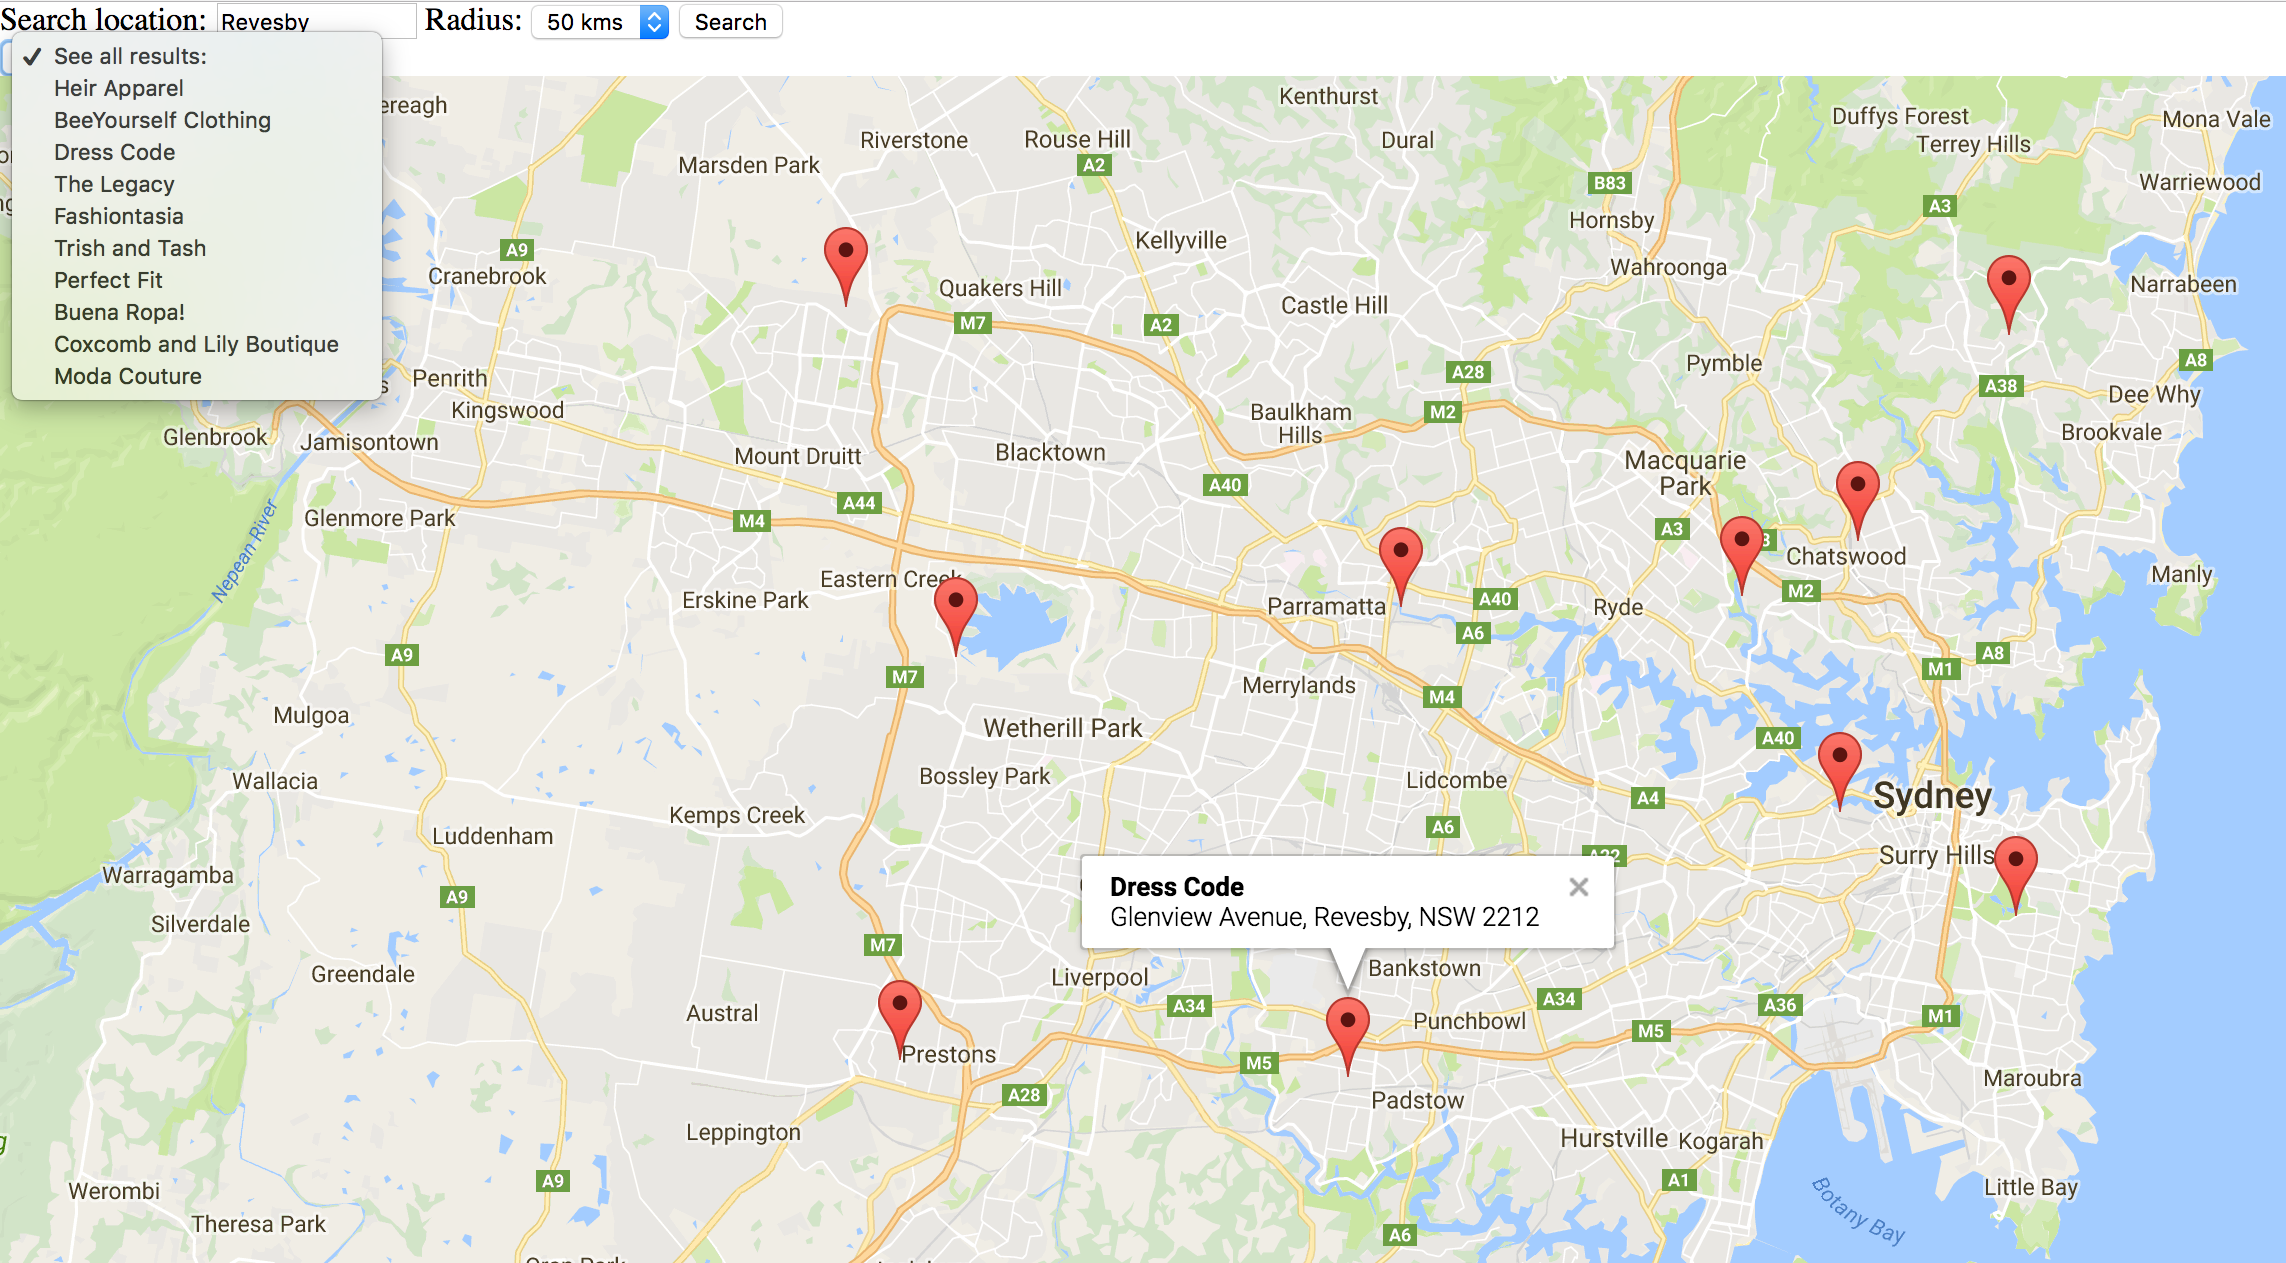
\includegraphics[scale=.17]{Capitulo2/images/geolocation}
	\caption{Ejemplo de uso de geolocalización a través del API de Google Maps}
	\label{fig:geolocation}
\end{figure}

Si una aplicación desea hacer uso de la geolocalización, esta deber ajustarse al estándar de Geolocalización de la W3C.

Dentro del estándar W3C, se definen los parámetros de información que pueden ser accedidos a partir del API Geolocation \citep{MarcoTeorico15}:
\begin{itemize}
	\item Accuracy: Representa la exactitud con la que fueron tomadas las últimas lecturas de la latitud y longitud del dispositivo con un 95\% de confianza.
	\item Altitude: Representa la cantidad en metros sobre la elipsoide WGS84.
	\item Altitude Accuracy: Representa la exactitud con la que fué tomada la última lectura de la altitud del dispositivo.
	\item Heading: Representa la dirección de desplazamiento en grados contando en el sentido de las agujas del reloj con respecto al norte verdadero en el rango de 0 <= rumbo <= 360.
	\item Latitude: Representa la coordenada de latitud de la geolocalización en grados decimales.
	\item Longitude: Representa la coordenada de longitud de la geolocalización en grados decimales.
	\item Speed: Representa la magnitud de la componente horizontal de la velocidad en metros por segundo.
\end{itemize}

 \paragraph{WGS84} El WGS84 (World Geodetic System 1984) es un sistema de coordenadas geográficas mundial que permite localizar cualquier punto de la Tierra (sin necesitar otro de referencia) por medio de tres unidades dadas (x,y,z). \citep{MarcoTeorico15}.

Se trata de un estándar en geodesia, cartografía, y navegación, que data de 1984. Tuvo varias revisiones (la última en 2004), y se considera válido hasta una próxima reunión (aún no definida en la página web oficial de la Agencia de Inteligencia Geoespacial). Se estima un error de cálculo menor a 2 cm, por lo que es en la que se basa el Sistema de Posicionamiento Global (GPS).